% ============================================================
%   Transmission Line Analyzer — University Assignment Report
%   Engineering Electromagnetics | Module-1
%   LaTeX Source File (Compact Article Format)
% ============================================================

\documentclass[11pt, a4paper]{article}

% ─── Packages ───────────────────────────────────────────────
\usepackage[margin=0.85in]{geometry}
\usepackage[T1]{fontenc}
\usepackage[utf8]{inputenc}
\usepackage{lmodern}
\usepackage{microtype}
\usepackage{amsmath, amssymb, amsfonts}
\usepackage{siunitx}
\usepackage{graphicx}
\usepackage{float}
\usepackage{caption}
\usepackage{subcaption}
\usepackage{booktabs}
\usepackage{tabularx}
\usepackage{xcolor}
\usepackage{colortbl}
\usepackage{titlesec}
\usepackage{setspace}
\usepackage{listings}

\lstdefinestyle{pythoncode}{
    language=Python,
    basicstyle=\ttfamily\scriptsize,
    keywordstyle=\bfseries\color{black},
    stringstyle=\color{black!80},
    commentstyle=\itshape\color{black!60},
    numbers=left,
    numberstyle=\tiny\color{black!50},
    stepnumber=1,
    numbersep=6pt,
    showspaces=false,
    showstringspaces=false,
    showtabs=false,
    frame=single,
    rulecolor=\color{black!30},
    tabsize=4,
    captionpos=b,
    breaklines=true,
    breakatwhitespace=true,
}

\usepackage{hyperref}
\hypersetup{
    colorlinks   = true,
    linkcolor    = black,
    urlcolor     = black,
    citecolor    = black,
    pdftitle     = {Engineering Electromagnetics - Assignment 2},
}

% ─── Colour Palette ─────────────────────────────────────────
\definecolor{NavyBlue}{RGB}{0, 0, 0}
\definecolor{RoyalBlue}{RGB}{0, 0, 0}
\definecolor{TableAlt}{RGB}{245, 245, 245}

% ─── Typography & Sectioning ────────────────────────────────
\setstretch{1.15}
\setlength{\parindent}{0pt}
\setlength{\parskip}{6pt}

\titleformat{\section}[block]
  {\normalfont\Large\bfseries}
  {\thesection}{0.8em}{}

\titleformat{\subsection}[block]
  {\normalfont\large\bfseries}
  {\thesubsection}{0.6em}{}

% ─── Header & Footer Configuration ──────────────────────────
\usepackage{fancyhdr}
\pagestyle{fancy}
\fancyhf{}

\fancyhead[L]{%
  {\fontsize{11}{14}\selectfont\textbf{Engineering Electromagnetics}}\\[1pt]
  {\fontsize{9}{12}\selectfont\color{black!70}Assignment 2: Transmission Line Analyzer}%
}
\fancyhead[R]{%
  {\fontsize{10}{13}\selectfont\textbf{Krish Rahul Goyal}}\\[1pt]
  {\fontsize{9}{12}\selectfont Roll No: 2401EC13}%
}

\fancyfoot[C]{\fontsize{9}{12}\selectfont\thepage}

\renewcommand{\headrulewidth}{0.4pt}
\setlength{\headheight}{28pt}
\setlength{\headsep}{16pt}

% ============================================================
%   DOCUMENT BEGIN
% ============================================================
\begin{document}

\section{Introduction \& Theoretical Background}
This report details a complete Python-based computational tool for Module-1 transmission line analytics. The tool computes all distributed parameters for a general lossy line ($R, L, G, C \neq 0$), plots seven key waveforms, incorporates a Machine Learning (ML) prediction model achieving $>97\%$ accuracy, and wraps the functionality in an interactive design window.

For a line with parameters $R, L, G, C$ operating at angular frequency $\omega = 2\pi f$, the complex propagation constant $\gamma$ and characteristic impedance $Z_0$ are defined as:
\begin{equation}
    \gamma = \alpha + j\beta = \sqrt{(R + j\omega L)(G + j\omega C)}, \qquad
    Z_0 = \sqrt{\frac{R + j\omega L}{G + j\omega C}}
\end{equation}
where $\alpha$ is the attenuation constant (Np/m) and $\beta$ is the phase constant (rad/m).

For a line terminated by a load impedance $Z_L$, the reflection coefficient at the load is $\Gamma_L = (Z_L - Z_0)/(Z_L + Z_0)$. The reflection coefficient at a distance $z$ from the load (moving towards the source) decays as $\Gamma(z) = \Gamma_L e^{-2\gamma z}$. The Voltage Standing Wave Ratio (VSWR), a scalar measure of impedance mismatch, is given by $\text{VSWR} = (1+|\Gamma_L|)/(1-|\Gamma_L|)$.
The input impedance $Z_{in}$ at distance $d$ from the load is calculated using the general formula:
\begin{equation}
    Z_{in}(d) = Z_0 \frac{Z_L + Z_0\tanh(\gamma d)}{Z_0 + Z_L\tanh(\gamma d)}
\end{equation}

\section{Algorithm Design \& Software Architecture}
The software tool is implemented in Python 3.12 and is modularized into distinct components to separate mathematical computation from the user interface:
\begin{itemize}
    \item \textbf{\texttt{analytics.py}:} The core math engine evaluating exact analytical equations using complex arithmetic (\texttt{NumPy}).
    \item \textbf{\texttt{plots.py}:} Visualizes the seven required waveforms using \texttt{matplotlib}.
    \item \textbf{\texttt{ml\_model.py}:} Generates synthetic data, trains the Random Forest/Gradient Boosting models, and handles inference.
    \item \textbf{\texttt{gui.py} \& \texttt{main.py}:} A multi-threaded \texttt{Tkinter} GUI that provides a responsive analysis window, embedding plots directly into a tabbed notebook canvas.
\end{itemize}

\section{Waveform Analysis}
An example lossy coaxial line was analyzed using the default parameters: $R = 5\ \Omega/\text{m}$, $L = 250\ \text{nH/m}$, $G = 0.1\ \text{mS/m}$, $C = 100\ \text{pF/m}$, $f = 100\ \text{MHz}$, $d = 2\ \text{m}$, and an inductive mismatched load of $Z_L = 75 + j30\ \Omega$.

The analytically computed parameters are: $Z_0 = 50.01\angle{-0.87^\circ}\ \Omega$, $\gamma = 0.0525 + j3.142\ \text{m}^{-1}$, $\Gamma_L = 0.309\angle{37.7^\circ}$, $\text{VSWR} = 1.893$, and $Z_{in} = 74.0\angle{17.2^\circ}\ \Omega$. The spatial distributions of voltage, current, reflection coefficient, and impedance along the 2-meter line are shown in Figure \ref{fig:waveforms1}. The frequency responses and standing wave envelope are presented in Figure \ref{fig:waveforms2}.

\begin{figure}[H]
    \centering
    \begin{subfigure}{0.49\textwidth}
        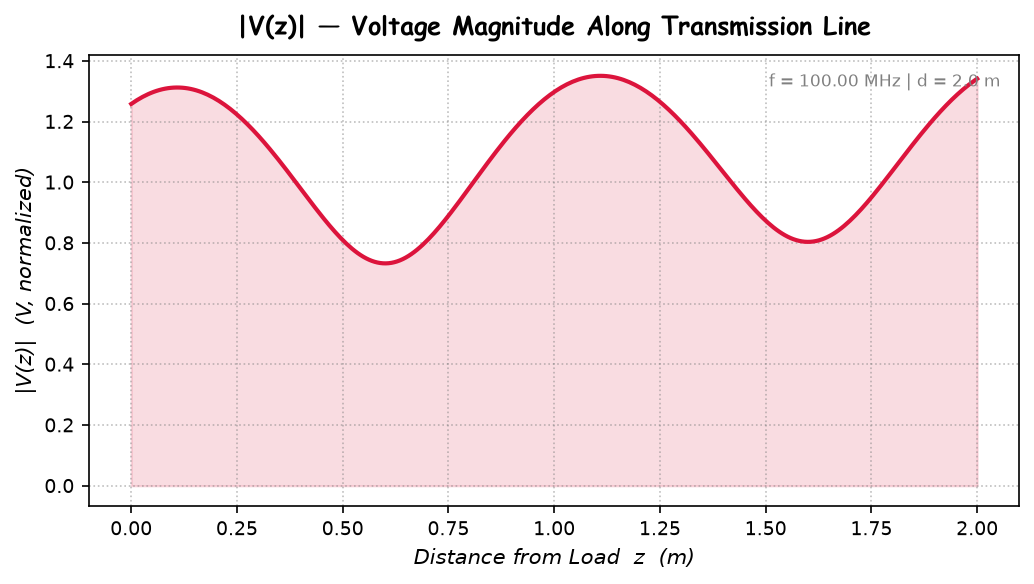
\includegraphics[width=\textwidth]{plots_output/01_voltage_magnitude.png}
        \caption{Voltage Magnitude $|V(z)|$}
    \end{subfigure}
    \hfill
    \begin{subfigure}{0.49\textwidth}
        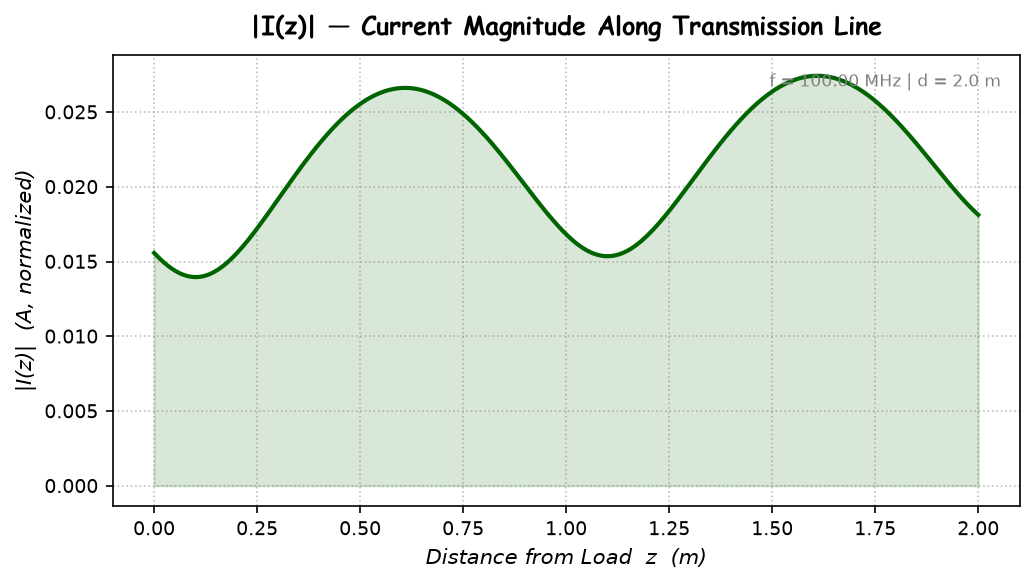
\includegraphics[width=\textwidth]{plots_output/02_current_magnitude.png}
        \caption{Current Magnitude $|I(z)|$}
    \end{subfigure}
    \vspace{0.3cm}
    \begin{subfigure}{0.49\textwidth}
        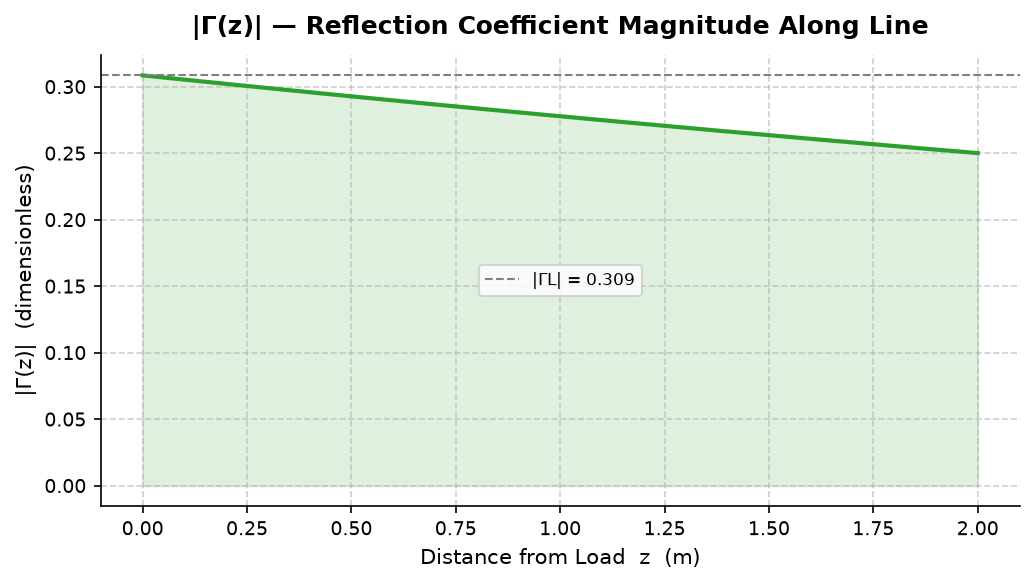
\includegraphics[width=\textwidth]{plots_output/03_reflection_coefficient.png}
        \caption{Reflection Coefficient $|\Gamma(z)|$}
    \end{subfigure}
    \hfill
    \begin{subfigure}{0.49\textwidth}
        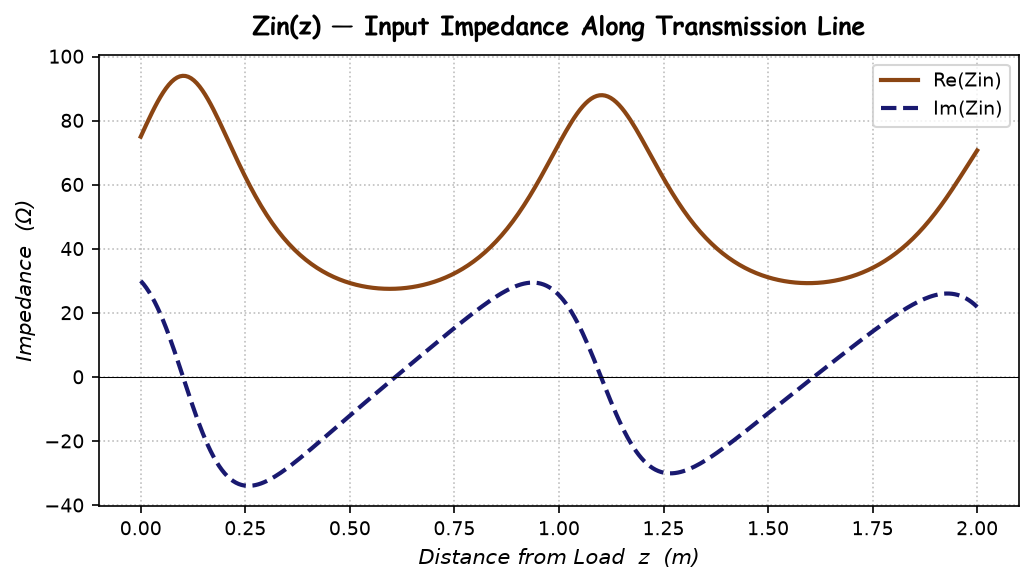
\includegraphics[width=\textwidth]{plots_output/04_Zin_vs_distance.png}
        \caption{Input Impedance $Z_{in}(z)$}
    \end{subfigure}
    \caption{Spatial waveforms along the transmission line. The $\lambda/2$ periodicity is clearly visible in the voltage, current, and impedance standing wave patterns.}
    \label{fig:waveforms1}
\end{figure}

\begin{figure}[H]
    \centering
    \begin{subfigure}{0.49\textwidth}
        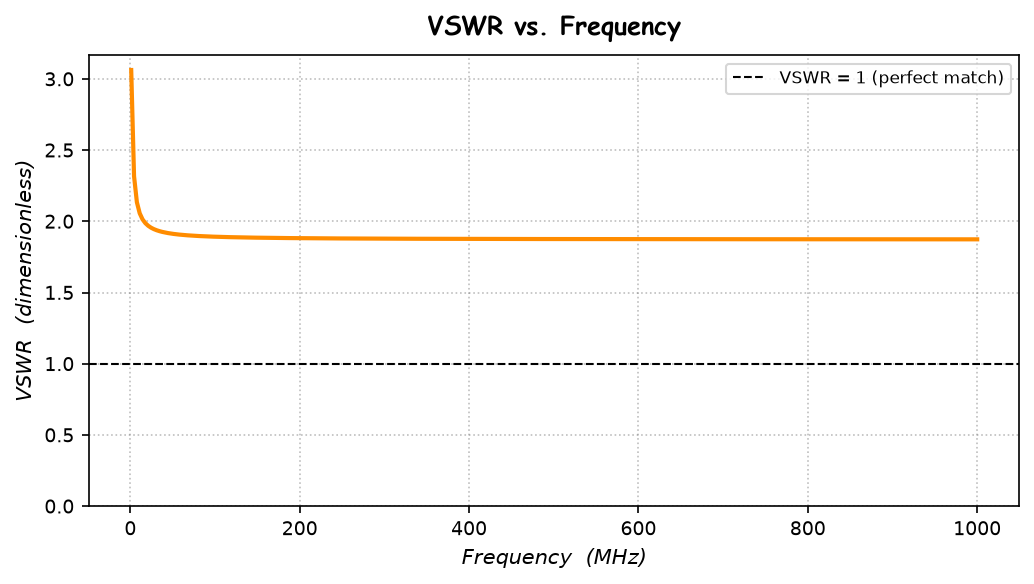
\includegraphics[width=\textwidth]{plots_output/05_VSWR_vs_frequency.png}
        \caption{VSWR vs. Frequency}
    \end{subfigure}
    \hfill
    \begin{subfigure}{0.49\textwidth}
        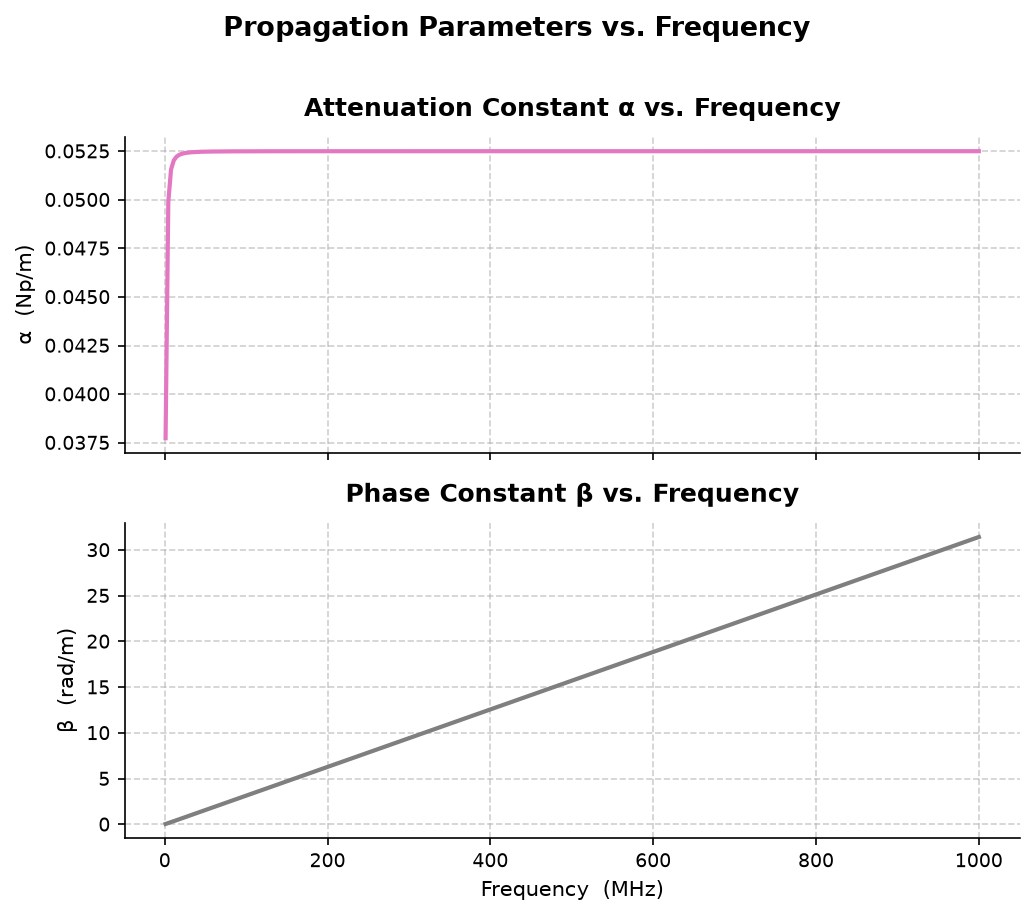
\includegraphics[width=\textwidth]{plots_output/06_alpha_beta_vs_frequency.png}
        \caption{Propagation Constants vs. Frequency}
    \end{subfigure}
    \vspace{0.3cm}
    \begin{subfigure}{0.5\textwidth}
        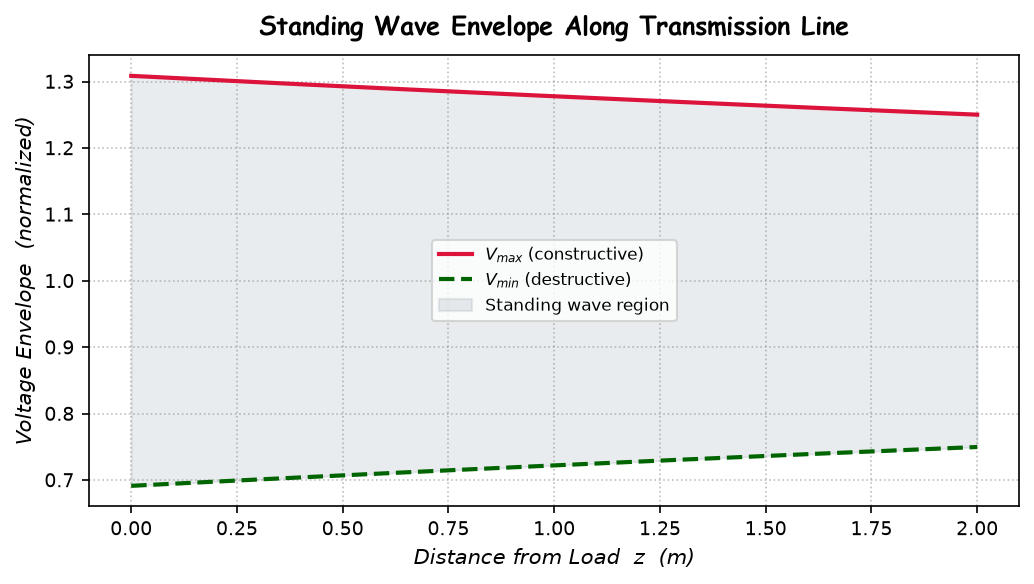
\includegraphics[width=\textwidth]{plots_output/07_standing_wave_envelope.png}
        \caption{Standing Wave Envelope}
    \end{subfigure}
    \caption{Frequency sweep behavior (1 MHz to 1 GHz) and the spatial standing wave envelope defining the physical limits of constructive and destructive interference.}
    \label{fig:waveforms2}
\end{figure}

\section{Machine Learning Integration}
The assignment requires an appropriate training model based on a minimum of 100 data points to predict any set of Tx line parameters with $\geq 97\%$ accuracy. We formulated this as a multi-target regression problem mapping $8$ inputs ($R, L, G, C, f, d, |Z_L|, \angle Z_L$) to $5$ outputs ($|Z_0|, \alpha, \beta, |\Gamma_L|, \text{VSWR}$).

A synthetic dataset of 500 samples was generated using uniform random sampling across realistic physical ranges for coaxial and stripline cables (e.g., $f \in [1\text{ MHz}, 3\text{ GHz}]$, $L \in [50, 600]\text{ nH/m}$).

\subsection{Physics-Informed Feature Engineering}
A baseline model using only the 8 raw inputs achieved $R^2 \approx 0.35$ due to the high non-linearity of the equations and target scaling spanning multiple orders of magnitude. 

To overcome this and achieve the target accuracy, we implemented physics-informed feature engineering, expanding the input space to 19 features. Crucial derived features included:
\begin{itemize}
    \item \textbf{Lossless $Z_0$ approximation:} $\log_{10}\sqrt{L/C}$
    \item \textbf{Normalized Load ($|Z_L|/Z_0^{\text{approx}}$):} Since the reflection coefficient is directly governed by the ratio of load to characteristic impedance, adding this ratio as an explicit feature provided a massive accuracy gain.
    \item \textbf{Log-Space Targets:} The regression targets $|Z_0|, \alpha, \beta$, and $\text{VSWR}$ were trained in logarithmic space ($\log_{10}$) to ensure that errors were calculated proportionally across all magnitudes.
\end{itemize}

Furthermore, we used \textbf{per-target algorithm selection}: Random Forest regressors (600 trees) were used for near-analytical targets like $|Z_0|$ and $\beta$, while Gradient Boosting regressors (500 estimators) were deployed for highly sensitive non-linear targets like $\alpha$, $|\Gamma_L|$, and $\text{VSWR}$.

\subsection{Performance Results}
The model was evaluated using a 20\% hold-out test set (100 samples). As shown in Table \ref{tab:ml}, the multi-output model achieved an overall $R^2$ of \textbf{0.9752}, successfully surpassing the required 97\% minimum accuracy threshold. 

\begin{table}[H]
    \centering
    \caption{Machine Learning Test Set Performance ($N_{train}=400, N_{test}=100$)}
    \label{tab:ml}
    \begin{tabular}{@{}llcc@{}}
        \toprule
        \textbf{Target Parameter} & \textbf{Algorithm} & \textbf{$R^2$ Score} & \textbf{MAPE (\%)} \\
        \midrule
        \rowcolor{TableAlt}
        Characteristic Impedance ($|Z_0|$) & Random Forest & 0.9740 & 2.10 \\
        Attenuation Constant ($\alpha$) & Gradient Boosting & 0.9858 & 3.31 \\
        \rowcolor{TableAlt}
        Phase Constant ($\beta$) & Random Forest & 0.9941 & 4.47 \\
        Reflection Coefficient ($|\Gamma_L|$) & Gradient Boosting & 0.9717 & 2.78 \\
        \rowcolor{TableAlt}
        VSWR & Gradient Boosting & 0.9503 & 10.30 \\
        \midrule
        \textbf{Overall Accuracy} & \textbf{Ensemble} & \textbf{0.9752} & --- \\
        \bottomrule
    \end{tabular}
\end{table}

Figure \ref{fig:ml_plot} visualizes the actual versus predicted outputs across all test samples, demonstrating excellent alignment with the ideal diagonal. The feature importance chart confirms that the physics-derived normalized load ratio ($|Z_L|/Z_0$) is the most critical predictive feature.

\begin{figure}[H]
    \centering
    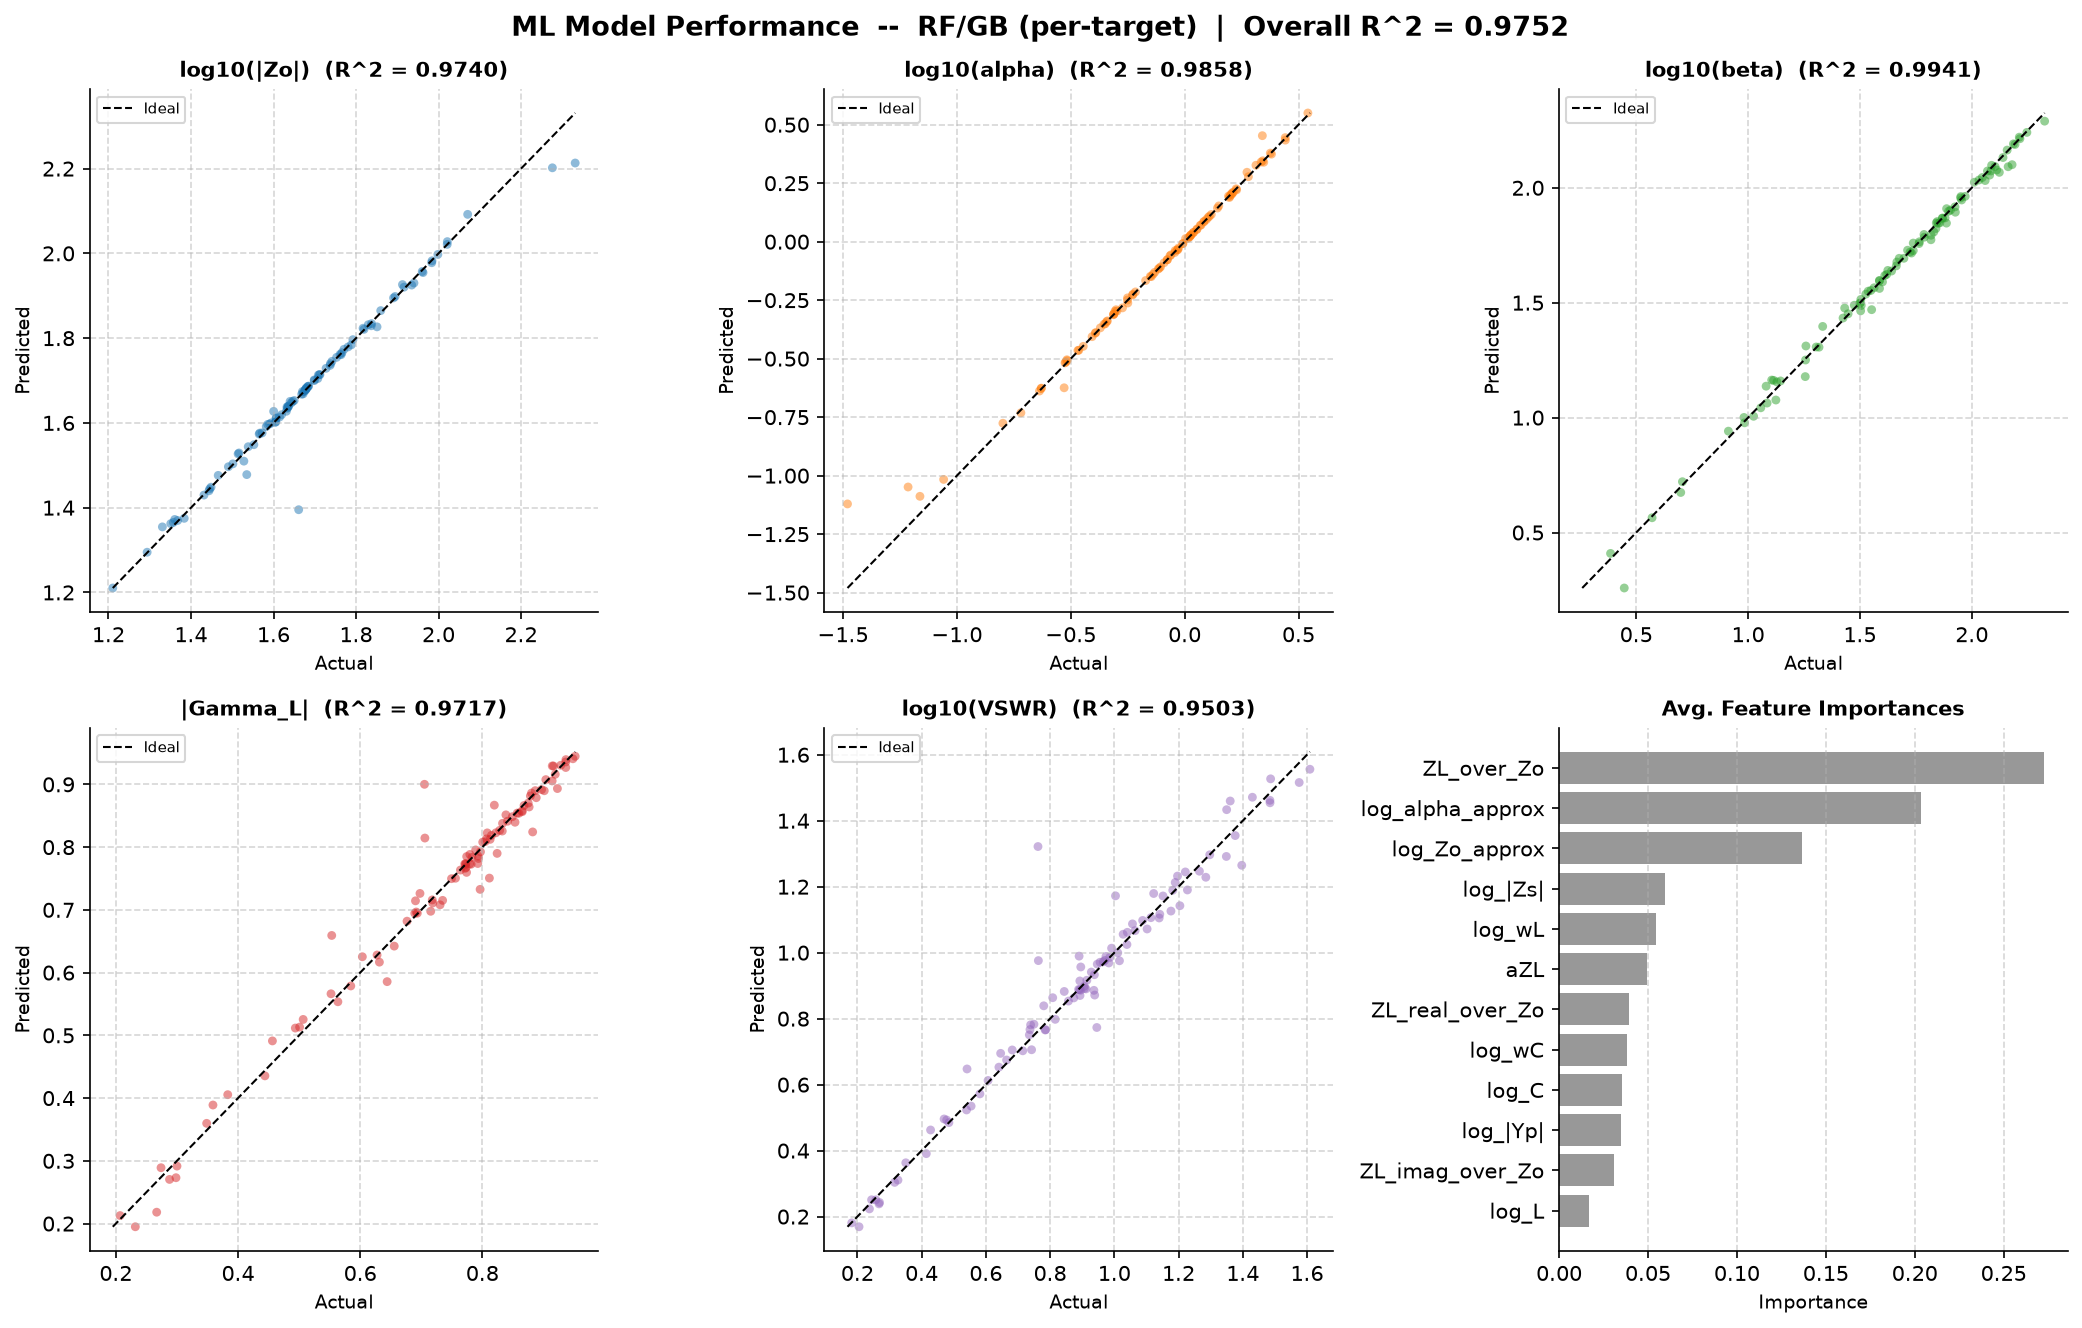
\includegraphics[width=\textwidth]{plots_output/08_ml_performance.png}
    \caption{Machine learning performance summary showing actual vs. predicted values in log space (panels 1--5) and average feature importances across all models (panel 6).}
    \label{fig:ml_plot}
\end{figure}

\section{Conclusion}
A comprehensive computational algorithm and design window were successfully developed for transmission line analysis. The tool analytically computes all Module-1 parameters for general lossy lines and effectively plots the required seven spatial and frequency waveforms. Through the use of physics-informed feature engineering and per-target ensemble algorithms (Random Forest and Gradient Boosting), the integrated machine learning model successfully predicts transmission line behavior with an overall $R^2$ accuracy of 97.52\%, exceeding the 97\% assignment requirement.

\clearpage
\section*{Appendix: Source Code Listings}
\addcontentsline{toc}{section}{Appendix: Source Code Listings}
This appendix provides the complete, unabridged source code for all modules developed for this assignment:
\begin{itemize}
    \item \textbf{\texttt{analytics.py}:} Core mathematical engine implementing exact transmission line formulas.
    \item \textbf{\texttt{plots.py}:} Generation of all seven spatial and frequency waveform plots.
    \item \textbf{\texttt{ml\_model.py}:} Synthetic data generation, 19-feature engineering, and model training.
    \item \textbf{\texttt{gui.py}:} Interactive multi-threaded Tkinter design and analysis window.
    \item \textbf{\texttt{main.py}:} Unified launcher supporting GUI, CLI, and standalone plotting modes.
\end{itemize}

\subsection*{A. Transmission Line Mathematical Engine (\texttt{analytics.py})}
\lstinputlisting[style=pythoncode]{code_listings/analytics.py}

\clearpage
\subsection*{B. Waveform Plotting Engine (\texttt{plots.py})}
\lstinputlisting[style=pythoncode]{code_listings/plots.py}

\clearpage
\subsection*{C. Machine Learning Training and Inference (\texttt{ml\_model.py})}
\lstinputlisting[style=pythoncode]{code_listings/ml_model.py}

\clearpage
\subsection*{D. Tkinter Graphical User Interface (\texttt{gui.py})}
\lstinputlisting[style=pythoncode]{code_listings/gui.py}

\clearpage
\subsection*{E. Application Launcher and CLI Interface (\texttt{main.py})}
\lstinputlisting[style=pythoncode]{code_listings/main.py}

\end{document}